\documentclass[11pt,a4paper,titlepage,twoside,openright]{report}
\usepackage[utf8]{inputenc}
\usepackage[T1]{fontenc}
\usepackage[spanish]{babel}
\usepackage[dvips]{graphicx}
\usepackage[nottoc,numbib]{tocbibind}
\usepackage{alltt}
\usepackage{amsmath}
\usepackage{amssymb}
\usepackage{color}
\usepackage{enumitem}
\usepackage{epsfig}
\usepackage{eurosym}
\usepackage{fancyhdr}
\usepackage{float}
\usepackage{graphics}
\usepackage{lettrine}
\usepackage{longtable}
\usepackage{mathpazo}
\usepackage[scaled=1.01]{inconsolata}
\usepackage{moreverb}
\usepackage{multirow}
\usepackage{pdfpages}
\usepackage{rotating}
\usepackage{sectsty}
\usepackage{subfigure}
\usepackage{tabu}
\usepackage{tabularx}
\usepackage{url}
\usepackage[hidelinks,pdftex,
            pdfauthor={Author Name},
            pdftitle={Project Title},
            pdfsubject={Trabajo de Fin de Grado},
            pdfkeywords={},
            pdfproducer={LaTeX},
            pdfcreator={pdflatex}]{hyperref}

\pagestyle{headings}

\setlength{\textwidth}{14.5cm}
\setlength{\textheight}{19.5cm}
\setlength{\oddsidemargin}{0.96cm}
\setlength{\evensidemargin}{0.46cm}
\setlength{\topmargin}{1.46cm}
\setlength{\footskip}{0.7cm}

\definecolor{udcpink}{RGB}{177,0,114}
\definecolor{udcgray}{RGB}{100,100,100}
\definecolor{irlabpink}{RGB}{241,92,135}
\definecolor{irlabblue}{RGB}{239,248,255}

%Doble espaciado
\renewcommand{\baselinestretch}{1.1}
\setlength{\parskip}{3pt}
\renewcommand*{\arraystretch}{1}

\hyphenation{Map-Reduce}
\hyphenation{shuffle}

% Title Page
\title{This is my title}
\author{I am the author}
\begin{document}
\def\tablename{Tabla}
\def\listtablename{Índice de Tablas}
\def\listfigurename{Índice de Figuras}

%%%%%%%%%%%%%%%%%%%%%%%%%%%%%%%%%%%%%%%%
% Portada
%%%%%%%%%%%%%%%%%%%%%%%%%%%%%%%%%%%%%%%%
\begin{titlepage}

\begin{center}
\hspace{36.5pt}\textcolor{udcgray}{{\fontfamily{phv}\selectfont Departamento de Computación}}\\\vspace{-2pt}
\hspace{4pt}\textcolor{udcpink}{{\fontfamily{phv}\selectfont Facultade de Informática}}\\\vspace{-5pt}

\includegraphics[scale=0.3]{img/udc}\\[35pt]
{\large TRABALLO DE FIN DE GRADO \\ GRADO EN ENXEÑERÍA INFORMÁTICA\\Mención en Sistemas de Información}\\[50pt]
\textbf{\begin{huge}Aplicación móvil para actividades a campo abierto\end{huge}
}\\[150pt]
\end{center}

\vspace{2cm}

\begin{flushright}
 \begin{tabular}{ll}
{\large {\bf Alumno:}}  & {\large Alberto Ramil Fernández}\\
{\large {\bf Directores:}} & {\large Javier Parapar López}\\
& {\large  Óscar Pedreira Fernández} \\
\end{tabular}\\
\vspace{0.5cm}
 {\large A Coruña, \today}
\end{flushright}

\end{titlepage}
\pagestyle{empty}
\cleardoublepage


%%%%%%%%%%%%%%%%%%%%%%%%%%%%%%%%%%%%%%%%
% Datos del trabajo
%%%%%%%%%%%%%%%%%%%%%%%%%%%%%%%%%%%%%%%%
\begin{titlepage}
\begin{Huge}{\bf Datos del trabajo}\end{Huge}\\
\newline

\begin{tabularx}{\textwidth}{XX}
\hline
{\large {\bf Título del Trabajo:}} & {\large Aplicación móvil para }\\
	& {\large actividades a campo abierto}\\
& \\
{\large {\bf Clase a la que pertenece:}} & {\large Trabajo Clásico de Ingeniería}\\
& \\
{\large {\bf Alumno:}}  & {\large Alberto Ramil Fernández }\\
& \\
{\large {\bf Directores:}} &{\large Javier Parapar López} \\
 &{\large Óscar Pedreira Fernández} \\\hline
\end{tabularx}

\vspace{1cm}

\begin{tabularx}{\textwidth}{ll}
\hline
{\large {\bf Miembros del tribunal:}}\\
\\
\\
\\
\\
\\
\\ \hline
\end{tabularx}

\vspace{1cm}

\begin{tabularx}{\textwidth}{XX}
\hline
{\large {\bf Fecha de lectura y defensa:}} & {\large A Coruña, \today}\\
\hline
\end{tabularx}

\vspace{1cm}

\begin{tabularx}{\textwidth}{XX}
\hline
{\large {\bf Calificación:}} & \\
\hline
\end{tabularx}

\end{titlepage}
\cleardoublepage


%%%%%%%%%%%%%%%%%%%%%%%%%%%%%%%%%%%%%%%%
% Certifico
%%%%%%%%%%%%%%%%%%%%%%%%%%%%%%%%%%%%%%%%
\begin{titlepage}
\pagestyle{empty}

\begin{minipage}[t][4cm][l]{.4\textwidth}
\begin{center}
{\sc Javier Parapar López}

Profesor de Universidad

Departamento de Computación

Universidade da Coruña
\end{center}
\end{minipage}
\begin{minipage}[t][4cm][l]{.1\textwidth}
\begin{center}
\vspace{1.2\baselineskip}
y
\end{center}
\end{minipage}
\begin{minipage}[t][4cm][l]{.4\textwidth}
\begin{center}
{\sc Óscar Pedreira Fernández}

Profesor Predoctoral FPU

Departamento de Computación

Universidade da Coruña
\end{center}
\end{minipage}

\vspace{2cm}

CERTIFICAN:
Que la memoria titulada {\it Aplicación móvil para actividades a campo abierto} ha sido realizada por {\sc Alberto Ramil Fernández} bajo su dirección y constituye su Traballo de Fin de Grado en el Grado de Enxeñería Informática.\\[4pt]
\begin{center}
En A Coruña, a \today
\end{center}

\vspace{3cm}

\begin{minipage}[t][5cm][l]{.45\textwidth}
\begin{center}
{\sc Javier Parapar López}

Director
\end{center}
\end{minipage}
\begin{minipage}[t][5cm][l]{.45\textwidth}
\begin{center}
{\sc Óscar Pedreira Fernández}

Director
\end{center}
\end{minipage}
\end{titlepage}
\cleardoublepage


%%%%%%%%%%%%%%%%%%%%%%%%%%%%%%%%%%%%%%%%
% Dedicatoria
%%%%%%%%%%%%%%%%%%%%%%%%%%%%%%%%%%%%%%%%
\begin{titlepage}
\vspace*{\stretch{1}}
\hfill \emph{Dedicatoria}
\vspace*{\stretch{1}}
\end{titlepage}
\cleardoublepage


%%%%%%%%%%%%%%%%%%%%%%%%%%%%%%%%%%%%%%%%
% Agradecimientos
%%%%%%%%%%%%%%%%%%%%%%%%%%%%%%%%%%%%%%%%
\begin{titlepage}
\vspace{2cm}
\begin{Huge}{\bf Agradecimientos}\end{Huge}\\
\newline


{\it
 A los profesores y ya amigos Javier Parapar López y Óscar Pedreira Fernández por su paciencia y ayuda a lo largo de este proyecto. Y que junto a Daniel Varcarce hicieron que cambiara mi rumbo en la carrera.\\
A mis padres por su paciencia.\\
A mis hermanos Rufo y Jara por aguantarme los fines de semana.\\
Y Arturo por su ayuda.
}
\\ 

\normalfont
\vspace{1cm}
\hfill{Alberto Ramón Ramil Fernández}

\hfill{A Coruña, \today}

\end{titlepage}
\cleardoublepage


%%%%%%%%%%%%%%%%%%%%%%%%%%%%%%%%%%%%%%%%
% Resumen
%%%%%%%%%%%%%%%%%%%%%%%%%%%%%%%%%%%%%%%%
\begin{titlepage}
\vspace{2cm}
\begin{Huge}{\bf Resumen}\end{Huge}\\
\newline
	El uso de dispositivos móviles en la vida cotidiana se ha ido incrementando exponencialmente en los últimos años. Como parte de esta tendencia, el uso de los dispositivos móviles se ha extendido a actividades como de ocio como al aire libre, como la pesca o la caza. En estas actividades, normalmente se necesita recordar puntos clave para poder volver a visitarlos en otras ocasiones, o las rutas seguidas para llegar a los mismos. Normalmente estas actividades se realizan en lugares de difícil acceso y un tanto peligrosos, bien por la peligrosa orografía de los accesos como del lugar en si mismo donde se practica.\\

Estos motivos nos llevaron a proponer este Trabajo de Fin de Grado.\\


El objetivo es desarrollar una aplicación móvil Android que permita al usuario realizar un seguimiento de sus jornadas tanto de caza como de pesca  y que le permita guardar sus puntos destacados para poder visitarlos en otras ocasiones. Además, la aplicación permitirá salidas en grupo, en las que cada usuario conocerá la posición de lo demás en todo momento. Poder monitorizar las jornadas conjuntamente siempre es un punto a favor en cuanto a la seguridad en estas actividades.\\



 La aplicación contará con una parte cliente(la propia aplicación nativa Android) y una parte servidor. La aplicación Android será la interfaz con la que que interactuará el usuario y en la que podrá visualizar toda la información. La parte servidora se encargará de almacenar los datos de forma persistente y de implementar los casos de uso. La comunicación entre ambas partes de llevará a cabo mediante servicios Web. En la aplicación móvil usaremos otros servicios propios de Android como Google Maps, Firebase y Location.\\



El proyecto seguirá la metodología ágil Scrum, que hará que éste esté dividido en una serie de Sprints. En cada Sprint  se llevarán a cabo trabajos de análisis, planificación, diseño, implementación y pruebas.\\

Todo lo anteriormente mencionado será recogido en esta memoria y comentado más profundamente.







\end{titlepage}
\cleardoublepage


%%%%%%%%%%%%%%%%%%%%%%%%%%%%%%%%%%%%%%%%
% Palabras clave
%%%%%%%%%%%%%%%%%%%%%%%%%%%%%%%%%%%%%%%%
\begin{titlepage}
\vspace{2cm}
\begin{Huge}{\bf Palabras clave}\end{Huge}\\
\newline

\begin{tabular}{c}
\hspace{10cm} \ \\
\end{tabular}\\
{\small \textsc{ First keyword, second keyword, etc.}}\\
\end{titlepage}
\cleardoublepage


%%%%%%%%%%%%%%%%%%%%%%%%%%%%%%%%%%%%%%%%
% Page style
%%%%%%%%%%%%%%%%%%%%%%%%%%%%%%%%%%%%%%%%
\pagestyle{fancy}
\renewcommand{\chaptermark}[1]{\markboth{
	 \MakeUppercase{\chaptername}\ \thechapter.\ \\ {\scriptsize #1}}{}}
\renewcommand{\sectionmark}[1]{\markright{
	 {\scriptsize \thesection\  #1}}{}}

\makeatletter
\def\cleardoublepage{\clearpage\if@twoside \ifodd\c@page\else
  \hbox{}\thispagestyle{empty}\newpage\if@twocolumn\hbox{}\newpage\fi\fi\fi}
\makeatother

%%%%%%%%%%%%%%%%%%%%%%%%%%%%%%%%%%%%%%%%
% Índice
%%%%%%%%%%%%%%%%%%%%%%%%%%%%%%%%%%%%%%%%
\tableofcontents


%%%%%%%%%%%%%%%%%%%%%%%%%%%%%%%%%%%%%%%%
% Capítulos
%%%%%%%%%%%%%%%%%%%%%%%%%%%%%%%%%%%%%%%%
\chapter{Introducción}
        \label{intro}
        En este primer capítulo de esta memoria se comentaran la motivación, los objetivos de la aplicación y la estructura de esta memoria. 
\section{Motivación}
Dado el creciente uso de los dispositivos móviles en los deportes al aire libre, como en caza y pesca, se aprecia una creciente demanda de aplicaciones que permitan el registro de estas actividades.\\

Uno de los aspectos más importantes de este tipo de actividades es la seguridad. Durante las jornadas de caza los cazadores caminan por el monte en grupos. Esto puede producir que en determinados momentos un cazador no conozca la situación de sus compañeros.
Esta aplicación permitirá conocer la ubicación de cada cazador en todo momento pudiendo minimizar accidentes por disparos fortuitos. Las jornadas de pesca en ocasiones  se realizan desde acantilados o lugares muy lejos de carreteras. Esto lleva a que, si tenemos una pequeña lesión, indicar nuestra ubicación a nuestros compañeros sea de gran ayuda.

Según datos del Consejo Superior de Deportes, en España  se tramitaron en el año 2016 343.130 licencias federativas de caza y 54.992 licencias de pesca. A estas personas son a las que iría dirigida esta aplicación. Cabe destacar que existen tanto cazadores como pescadores que realizan sus actividades sin tener que estar federados, por lo que el número de licencias federativas aumentaría. 





Por todo esto se propone este Trabajo de Fin de Grado.
El objetivo de este proyecto será diseñar y construir una herramienta que permita gestionar las actividades a campo abierto como
caza y pesca, permitiendo mediante geolocalización guardar los puntos de interés, las rutas seguidas,
llevar control de los usuarios presentes, guardar información de los éxitos de las jornadas y poder realizar jornadas de caza y pesca con un seguimiento  total de nuestros compañeros.


\section{Objetivos}
El objetivo es desarrollar una aplicación móvil en Android que permita al usuario realizar un seguimiento de sus jornadas tanto de caza como de pesca  y que le permita guardar sus puntos destacados para poder visitarlos en otras ocasiones. Sin olvidar que el poder monitorizar la jornadas conjuntamente siempre es un punto a favor para seguridad de los participantes en estas actividades.\\ 
Los principales objetivos serán:

\begin{itemize}
\item Registro de usuarios y adición de amigos a usuario.
\item El usuario podrá conocer su ubicación en tiempo real en un mapa.
\item El usuario podrá comenzar y parar una jornada.
\item El usuario podrá visualizar la ruta seguida durante la jornada.
\item Administrar puntos clave para el usuario.
\item Clasificación de los puntos de interés según su tipología.
\item Visualizar dichos puntos en un mapa.
\item Gestionar grupos de usuarios participantes en la jornada y poder ver su ubicación en tiempo
real.

\end{itemize}


\section{Estructura de la memoria}
La memoria del presente proyecto está estructurada del siguiente modo:

\begin{itemize}
\item \textbf{Introducción.} Contextualiza el proyecto, introduce el tema a tratar y detalla los objetivos del mismo desde un punto de vista global.
 También comenta la estructura de la memoria.

\item \textbf{Tecnología.} Describe y justifica las principales tecnologías empleadas para desarrollar el proyecto.



\item \textbf{Proceso de ingeniería.} Detallamos el proceso de ingeniería: la metodología empleada,como funciona, la adaptación de la misma y los participantes.


\item \textbf{Análisis.} Comentamos las funcionalidades de la aplicación, describiendo más detenidamente los casos de uso y requisitos. 
\item \textbf{Seguimiento.} Comentamos las fases que pasa el proyecto usando la metodología Scrum.
\item \textbf{Diseño.} Describimos la arquitectura del proyecto.
\item \textbf{Implementación.} Describiremos aspectos concretos destacados de la implementación y las pruebas realizadas.





\item \textbf{Conclusiones y trabajo futuro}
Comentamos el producto obtenido y futuros cambios que se podrían realizar.



\end{itemize}

\section{Estudio de mercado}
En esta sección comentaremos otras aplicaciones que presentan funcionalidades similares a las de este trabajo de fin de grado.



\subsection{iHunt Journal}

iHunt Journal es una aplicación de software de cacería que presenta las siguientes características: 
\begin{itemize}
\item Ver puntos en el mapa, figura \ref{fig:iHunt1}
\item Guardar puntos en un mapa,figura \ref{fig:iHunt2}
\item Puede grabar sus búsquedas.
\item Graba  estadísticas.
\item Permite planificar las próximas cacerías según meteorología, figura \ref{fig:iHunt3}.
\item Puede grabar sus trofeos figura \ref{fig:iHunt4}.

\end{itemize}

\begin{figure}[htbp]
\begin{minipage}[b]{0.5\linewidth} %Una minipágina que cubre la mitad de la página
\centering
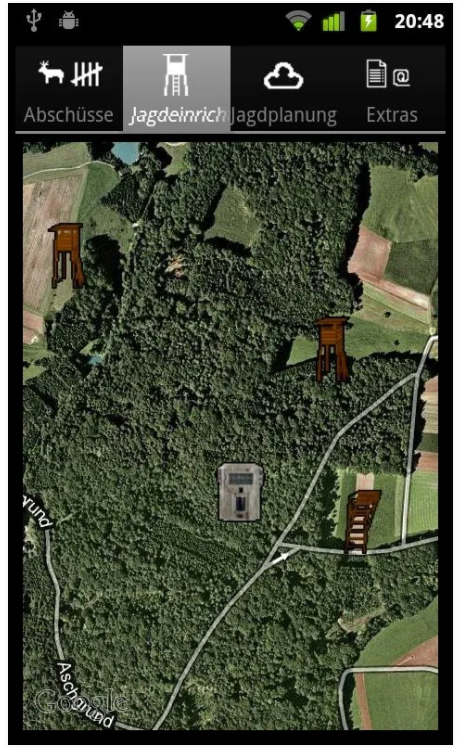
\includegraphics[width=6cm]{iHunt1.png}
\caption{ Visualizar mapa con iHunt}
\label{fig:iHunt1}
\end{minipage}
\hspace{0.5cm} % Si queremos tener un poco de espacio entre las dos figuras
\begin{minipage}[b]{0.5\linewidth}
\centering
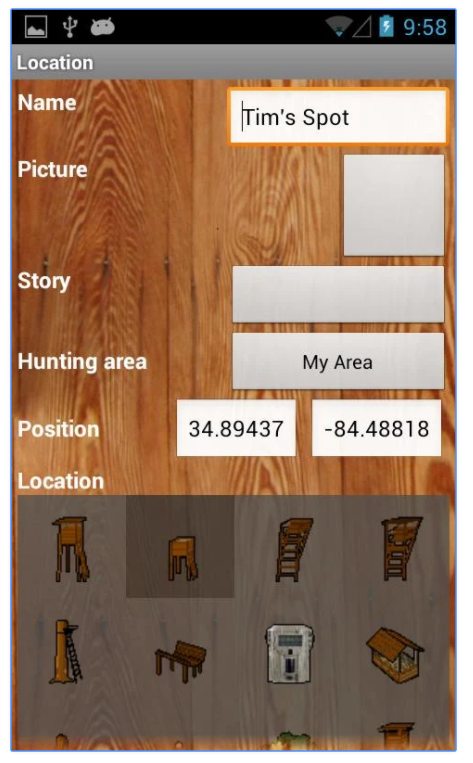
\includegraphics[width=6cm]{iHunt2.png}

\caption{Registro de un punto con iHunt}
\label{fig:iHunt2}
\end{minipage}
\begin{minipage}[b]{0.5\linewidth}
\centering
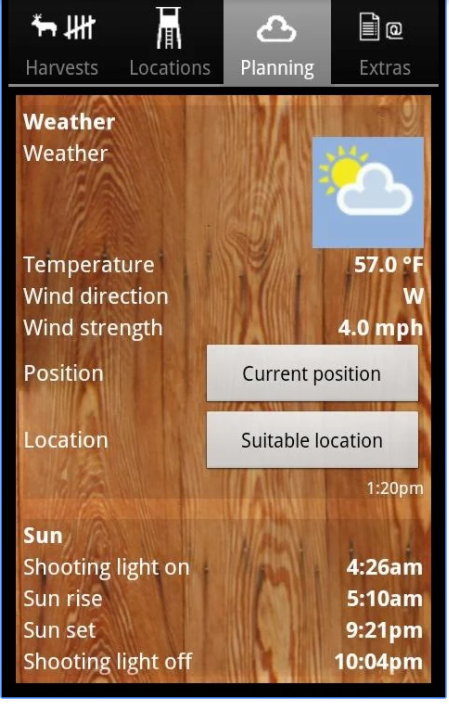
\includegraphics[width=6cm]{iHunt3.png}

\caption{Planificación con iHunt}
\label{fig:iHunt3}
\end{minipage}
\begin{minipage}[b]{0.5\linewidth}
\centering
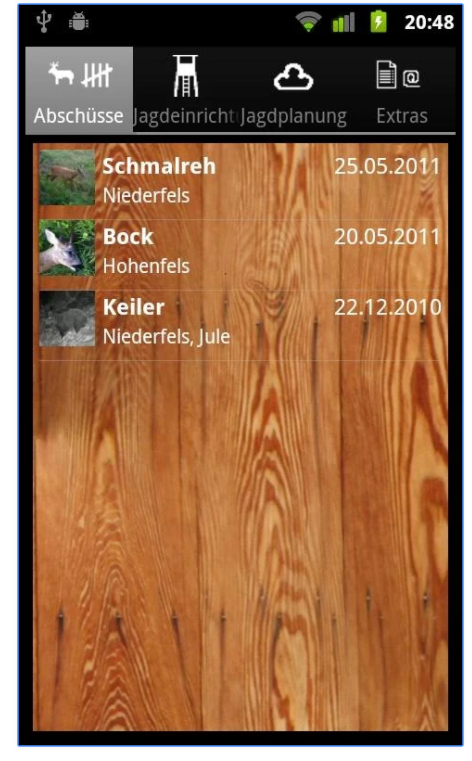
\includegraphics[width=6cm]{iHunt4.png}

\caption{Registro de trofeo con iHunt}
\label{fig:iHunt4}
\end{minipage}
\end{figure}

iHunt Journal está disponible desde iPhone y Android .


\subsection{My Fishing Companion}
 My Fishing Companion se trata de una aplicación para salir de pesca para Smartphone Android. Nos da la posibilidad de:
\begin{itemize}
\item Localizar nuestros lugares de capturas  véase figura \ref{fig:pesca2}
 \item Añadir vídeos y fotos
 \item 	Ver el tiempo que nos espera véase figura \ref{fig:pesca4}
  \item  Marcar capturas  véase figura \ref{fig:pesca3}
\end{itemize} 
 
 
 También es interesante la comunidad en la que se comparten todos estos datos y que te pueden ayudar a elegir el mejor lugar y el mejor día de pesca.
 
 \begin{figure}[htbp]
\begin{minipage}[b]{0.5\linewidth} %Una minipágina que cubre la mitad de la página
\centering
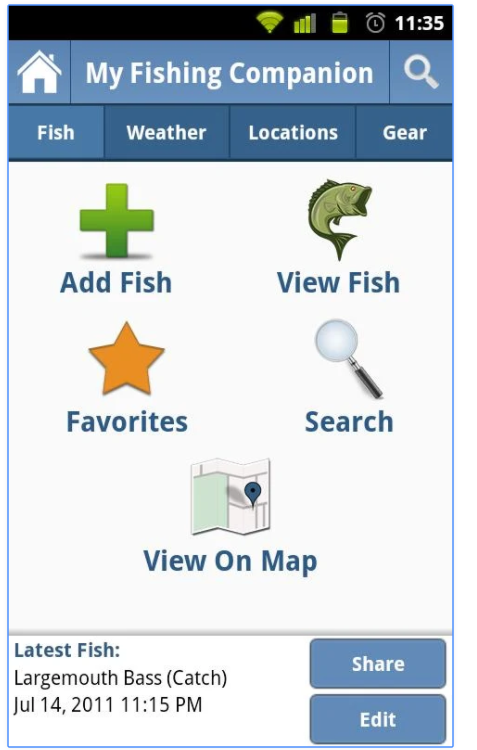
\includegraphics[width=6cm]{pesca1.png}
\caption{ Opciones de la aplicación}
\label{fig:pesca1}
\end{minipage}
\hspace{0.5cm} % Si queremos tener un poco de espacio entre las dos figuras
\begin{minipage}[b]{0.5\linewidth}
\centering
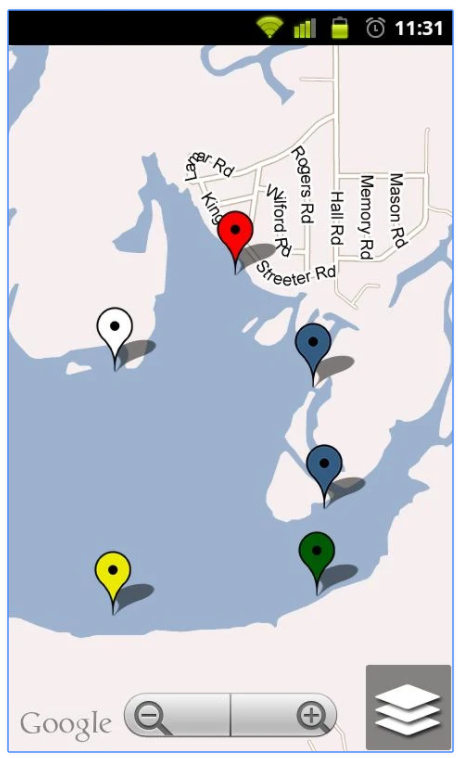
\includegraphics[width=6cm]{pesca2.png}

\caption{Puntos de pesca guardados}
\label{fig:pesca2}
\end{minipage}
\begin{minipage}[b]{0.5\linewidth}
\centering
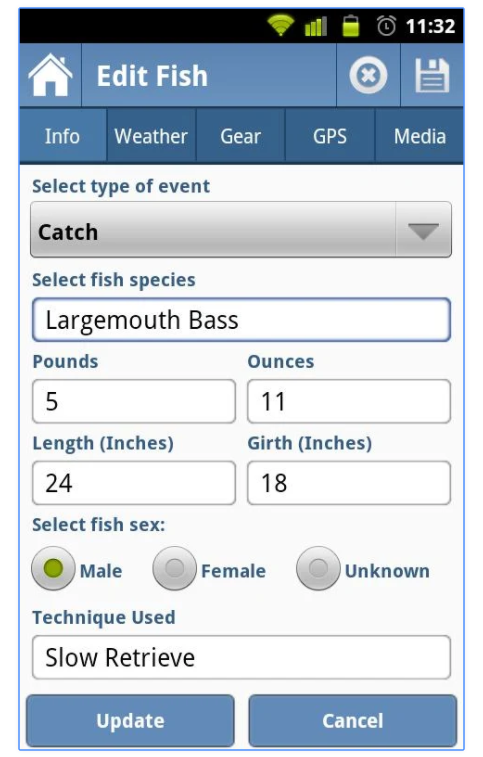
\includegraphics[width=6cm]{pesca3.png}

\caption{Datos de una captura}
\label{fig:pesca3}
\end{minipage}
\begin{minipage}[b]{0.5\linewidth}
\centering
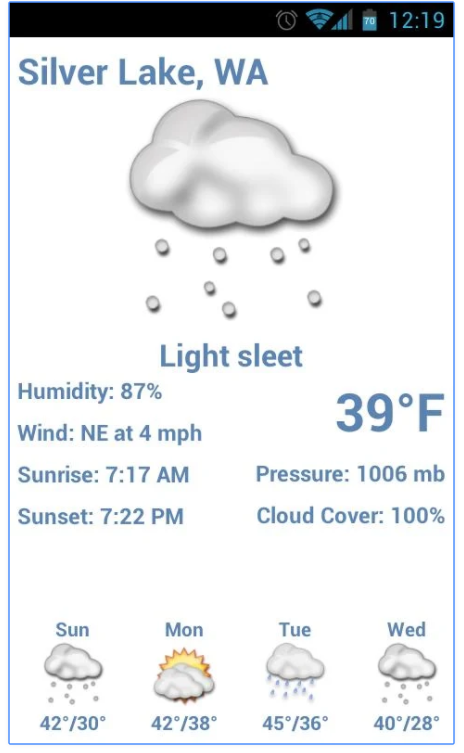
\includegraphics[width=6cm]{pesca4.png}

\caption{Datos sobre la meteorología}
\label{fig:pesca4}
\end{minipage}
\end{figure}
        \cleardoublepage

\chapter{Conceptos}
        \label{concept}
        \input{subfiles/conceptos}
        \cleardoublepage

\chapter{Tecnología}
        \label{tec}
        
Una buena elección de la tecnología será una condición necesaria, aunque no suficiente, para llevar a cabo un proyecto con éxito.

En este capítulo presentamos las tecnologías utilizadas en el desarrollo de este proyecto. 
\section{Android SDK}
Android  \cite{2}  \cite{3} es un sistema operativo especialmente diseñado para dispositivos móviles. Permite el desarrollo de sus aplicaciones en un lenguaje similar al Java. El sistema operativo nos proporciona de manera sencilla todas las inferfaces para el desarrollo de las aplicaciones que puedan acceder a las funciones del teléfono.\\

\textbf{Android SDK}\\

El SDK de Android ofrece un conjunto de herramientas para el desarrollo de aplicaciones incluyendo:
\begin{itemize}
\item \textbf{Depurador de código}
\item \textbf{Simulador de dispositivos de la plataforma. basado en QEMU}. Siendo QEMU  un emulador de procesadores. 
\item\textbf{ Bibliotecas.}
\item \textbf{Documentación.}
\item \textbf{Ejemplos de código.}

\end{itemize}


\section{Eclipse }


Eclipse es un IDE en Java para
( ver Figura~\ref{fig:eclipse}) para el desarrollo de software. Fue creado por IBM como sucesor de una de sus herramientas y ahora está en manos de la Fundación Eclipse que es quien se encarga de seguir desarrollándolo.
Se decidió usar esta herramienta de desarrollo ya que es totalmente gratuita por lo que no encarece el precio del proyecto y porque el entorno que usamos en Android esta basado en este.  
\begin{figure}[H]
		\centering
		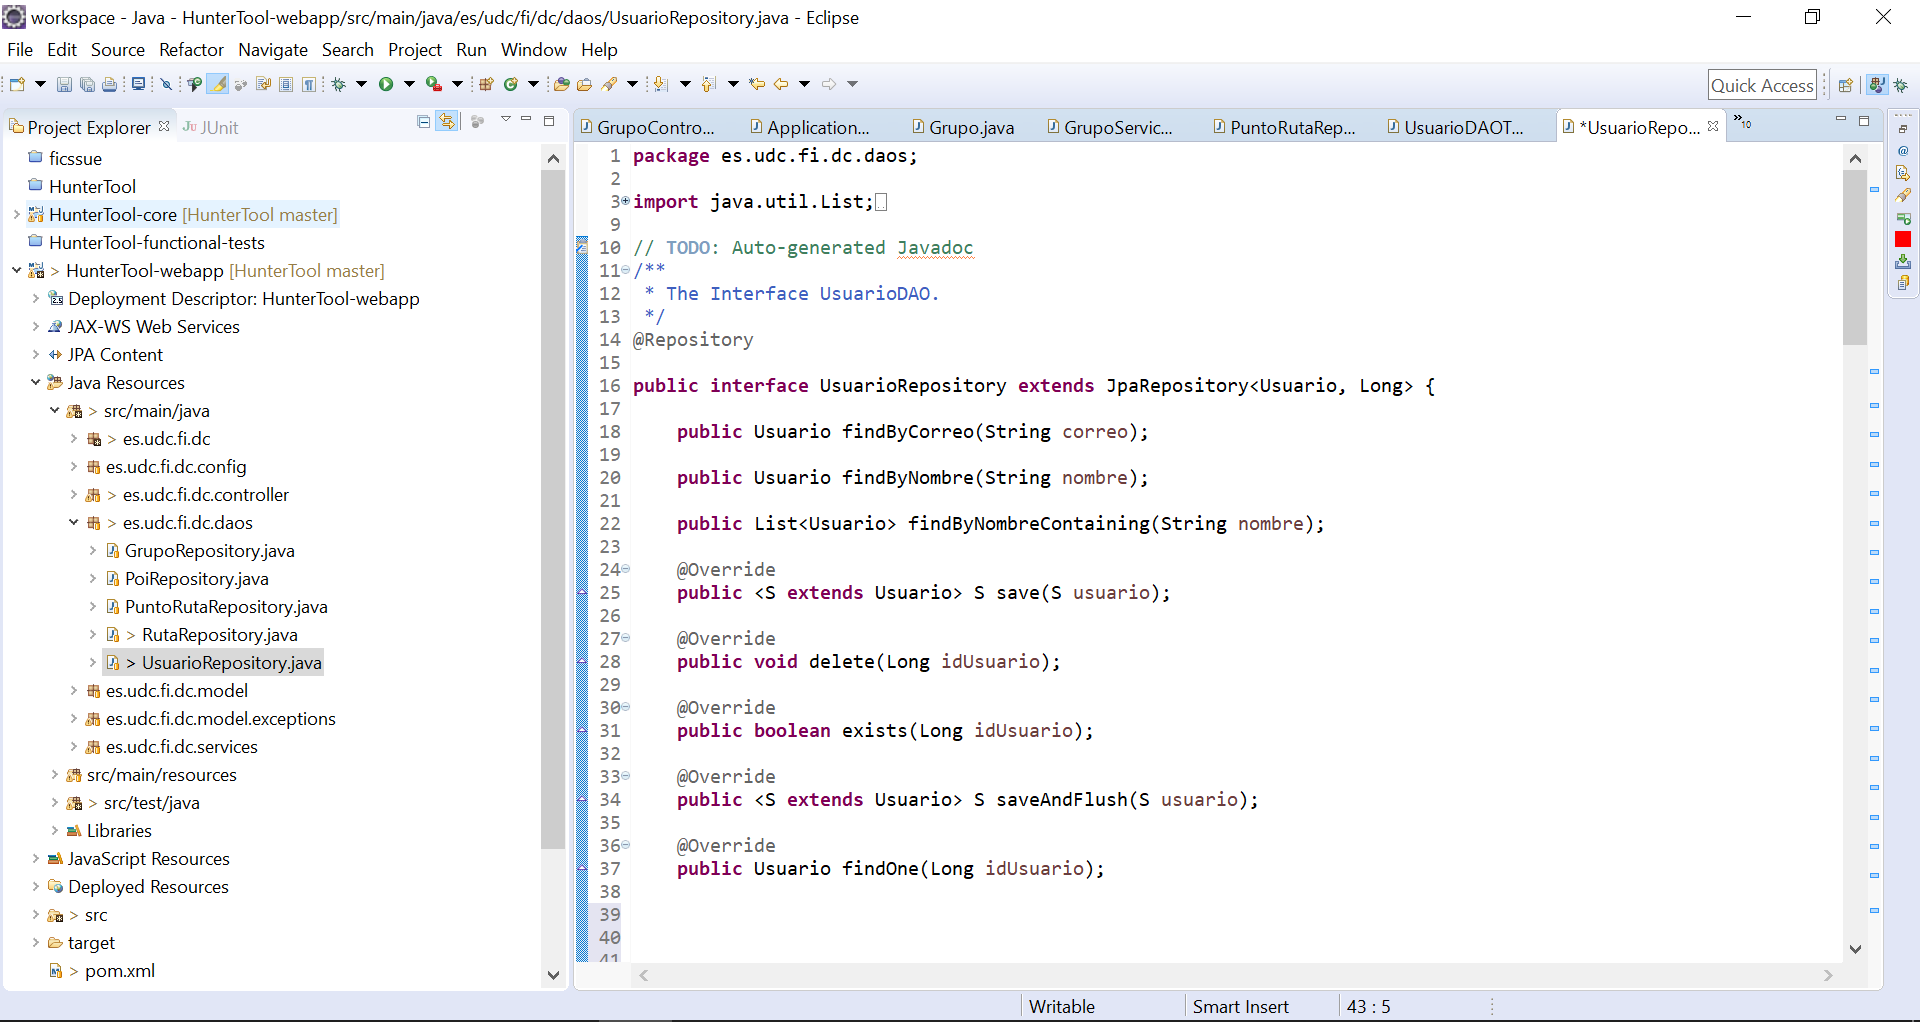
\includegraphics[width=\textwidth] {eclipse.png}
		\caption{Entorno de trabajo Eclipse }
		\label{fig:eclipse}
	\end{figure}
	
	
	
\section{Spring}
Spring es un framework de código abierto que tiene como objetivo ayudar al desarrollador a trabajar con otras APIs de manera más sencilla. Nos proporciona un modelo de programación y configuración integral para aplicaciones empresariales basadas en Java, en cualquier tipo de plataforma de implementación. 
	
Las funcionalidades principales que ofrece y por ello elegí, serían:

\begin{itemize}
\item \textbf{Programación orientada aspectos},paradigma que nos ayuda a eliminar dependencias entre módulos acortando las líneas de código de los servicios para así poder centrarnos en la lógica de la aplicación. Lo que conlleva reducir  la probabilidad de errores en la codificación o ineficiencias.


\item\textbf{ Inyección de dependencias}, patrón que ayuda a reducir el acoplamiento entre los distintos componentes de la aplicación. Esto lo consigue haciendo que una clase le proporcione a otra sus dependencias haciendo que la otra no tenga que crearlas ella misma. De este modo a través de un interfaz una clase tienes las dependencias de otra sin tener que preocuparse de la implementación de las mismas, lo que es favorable para reducir el acoplamiento.





\begin{lstlisting}[language=java,
 ,backgroundcolor=\color{backcolour},   
    commentstyle=\color{codegreen},
    keywordstyle=\color{magenta},
    numberstyle=\tiny\color{codegray},
    stringstyle=\color{codepurple}]  
@Service
public class GrupoServiceImpl implements GrupoService {

	@Autowired
	GrupoRepository grupoDAO;

	public void setGrupoDAO(GrupoRepository grupoDAO) {
		this.grupoDAO = grupoDAO;
	}


\end{lstlisting} 



\end{itemize}


\section{Android Studio}
Android Studio es el entorno de desarrollo integrado (IDE)  oficial para Android que nos ofrece las herramientas más rápidas para crear apps en todas las clases de dispositivos Android.
Además de ser una potente herramienta para la creación de código permite:

\begin{itemize}
\item Realizar compilaciones  de nuestro código para comprobar el estado de nuestras variables en los puntos que nosotros le indiquemos sin necesidad de general un APK.
\begin{figure}
		\centering
		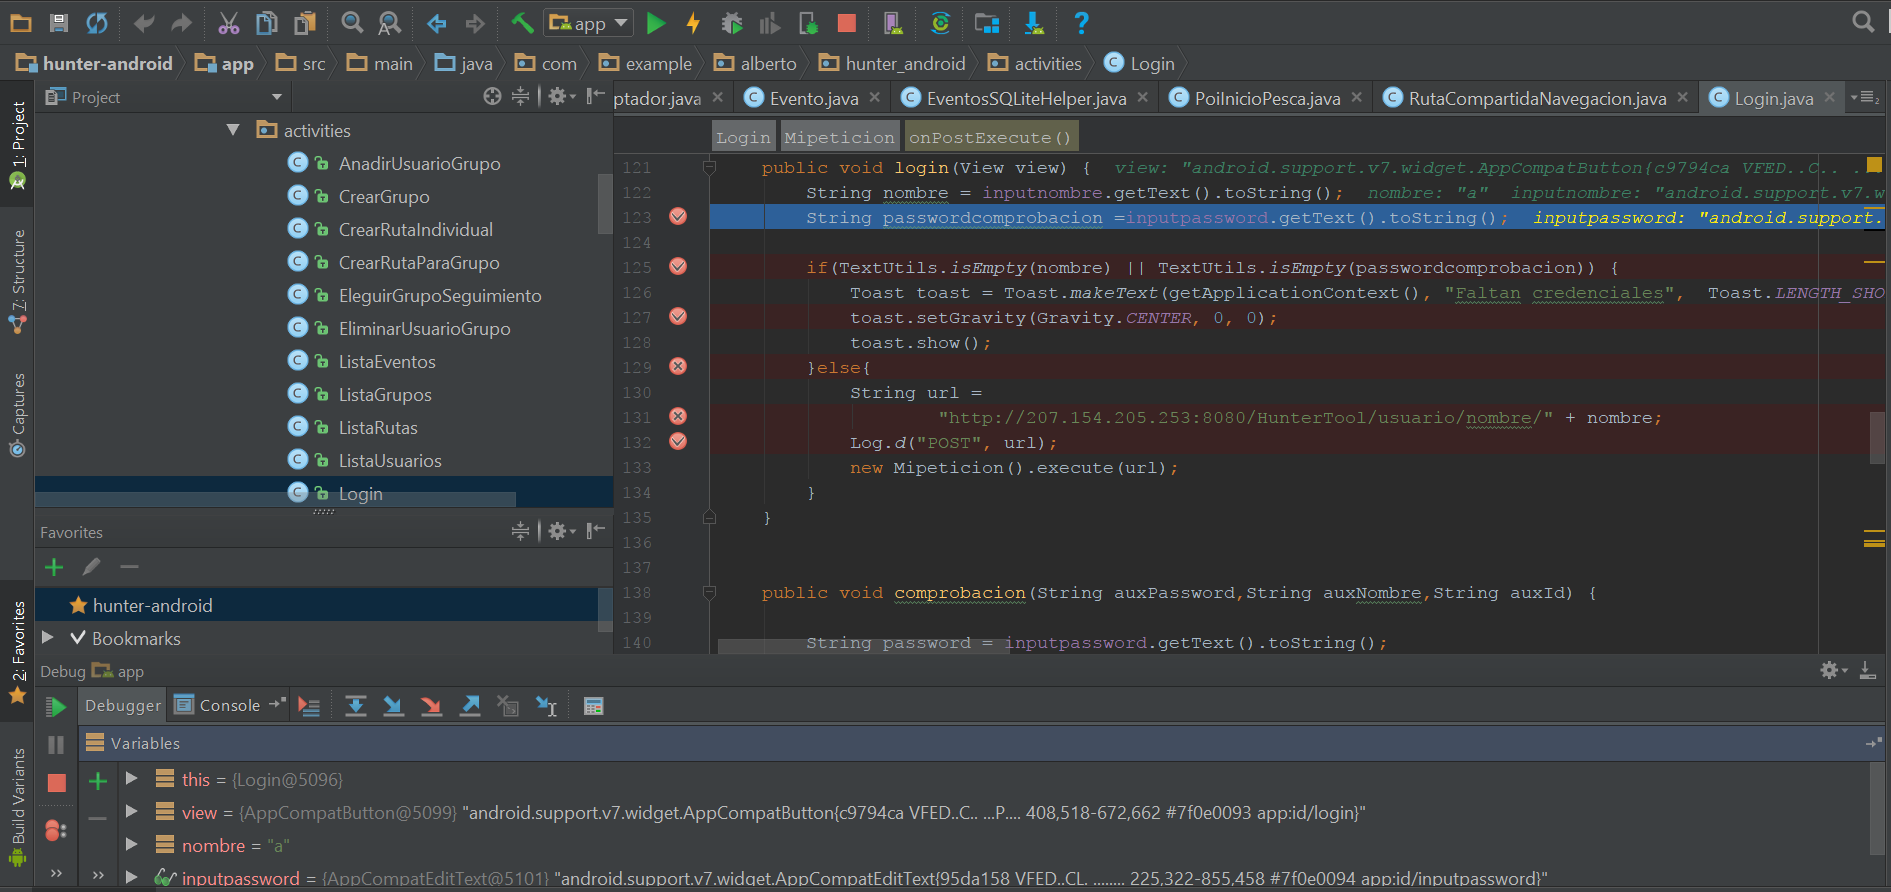
\includegraphics[width=\textwidth] {debug.png}
		\caption{Captura de pantalla realizando app debug }\label{fig:debug}
	\end{figure}

\item Generar un APK (Android Application Package) para la ejecución de nuestra aplicación móvil tanto de forma simulada, ayudándonos del simulador que nos proporciona o usando un móvil.
\end{itemize}
\begin{figure}
		\centering
		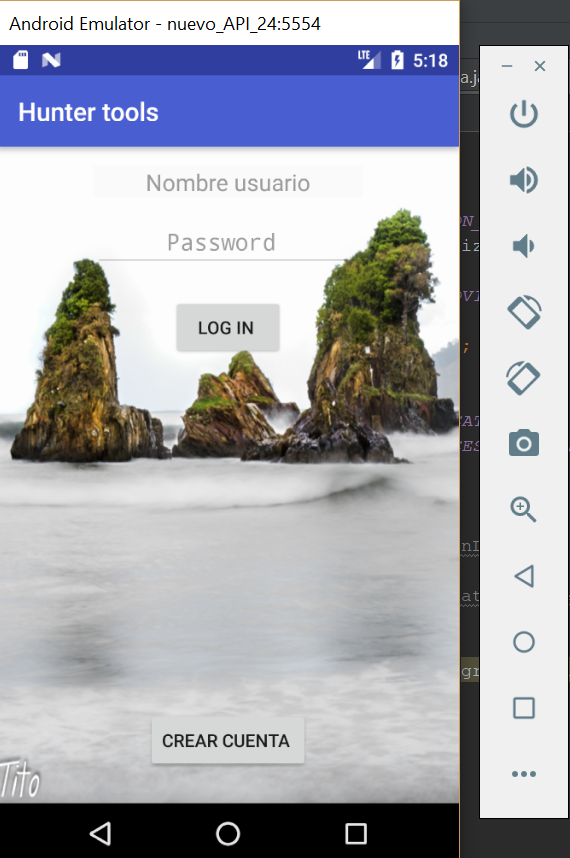
\includegraphics[width=0.6\textwidth] {emulador.png}
		\caption{Emulador de Android con mi aplicación}
		\label{fig:emulador}
	\end{figure}
 



\section{Git}
Git es un software para ayudarnos con el control de versiones  pensado para el mantenimiento de múltiples versiones de aplicaciones cuando estas tienen un número muy alto de archivos y queremos poder volver a un punto anterior o como copias de seguridad. A su vez, Git ofrece dos opciones para el control de versiones, una mediante un interfaz y otra mediante línea de comandos. Se escogió esta opción por las facilidades de uso que ofrece a la hora de realizar lo commits y el fácil nombrado de los mismos cuando queremos actualizar el repositorio.
\section{Maven}
Maven es una herramienta de software para la gestión y construcción de proyectos Java.
 Maven utiliza un Project Object Model (POM) en formato
XML para describir sus dependencias con otros módulos como jpa, firebase o postgrest. Viene con objetivos predefinidos para la compilación del código o su empaquetado. Se escogió por la buena estructuración de los paquetes que genera y por las similitudes que presenta frente al Gradle que usaremos en el entorno de desarrollo Android Studio.




\section{Gradle}
Gradle es una herramienta de software para la gestión, construcción de proyectos Android y gestor de dependencias. Ofrece
  herramientas de compilación avanzadas, para automatizar y administrar el proceso de compilación, y al mismo tiempo te permite definir configuraciones de compilación personalizadas.



\section{Jackson}

Jackson es un parseador para el desarrollo de Servicios Web en java. Implementa un conjunto de   herramientas de procesamiento de datos para Java haciendo que el desarrollo de servicios Rest sean más simples. Se eligió esta opción por lo sencillo que hacia el mapeo de objetos en las peticiones a JSON y dado que se usa el framework Spring este parseador ya viene integrado.








\section{JPA/Hibernate}
Hibernate es una herramienta de mapeo objeto-relacional para la plataforma Java que ayuda a la transformación de objetos del modelo a una entidad de la base de datos persistente. Este mapeo ayuda a  no tener que definir la entidad directamente en nuestro gestor de base de datos. Para conseguir esto debemos usar las anotaciones pertinentes en el entorno de desarrollo (Eclipse) sin necesidad de acceder al gestor de base de datos en ningún momento. Una vez puestas las anotaciones los accesos a datos de la  bases de datos pasan a ser muy sencillos.





\section{PostgreSQL}
PostgreSQL es un gestor de bases de datos objecto-relacional  que permite trabajar con grandes cargas de datos consiguiendo una tolerancia alta a errores.
Se decidió usar este gestor porque tiene una gran adaptabilidad a otros entornos de trabajo lo que ayuda a ganar agilidad y eficiencia. También nos proporciona  el PgAdmin que facilita la gestión y administración de bases de datos ya sea mediante instrucciones SQL o con ayuda de un entorno gráfico. Permite acceder a todas las funcionalidades de la base de datos, consulta, manipulación y gestión de datos.
\section{JUnit}
JUnit es el framework de testing para Java más extendido.
Permite la ejecución de clases Java para evaluar el comportamiento de los métodos a testar.


\vspace{1cm}

Con estas tecnologías se ha llevado a cabo la construcción de los distintos componentes del sistema siguiendo los pasos que comentaremos en el próximo capítulo.

        \cleardoublepage

\chapter{Proceso de ingeniería}
		\label{ing}
		En este capítulo se justifica la elección y se describe la metodología de desarrollo sobre la que se apoya el proceso de ingeniería. En este proyecto se ha empleado una metodología ágil, Scrum. 



\section{Scrum}

El Scrum es una  Metodología ágil \cite{6} \cite{9} que se usa para estructurar y gestionar proyectos, y para minimizar los riesgos durante la realización del mismo.
Esta metodología esta basada en ciclos iterativos cortos e incrementales, lo que se traduce en una gran flexibilidad a la hora de adaptarse a cambios que surjan duran el desarrollo del proyecto.
Entre las ventajas de Scrum se encuentran la baja carga de burocracia y documentación, productividad, calidad y que se realiza un seguimiento diario de los avances del proyecto, logrando una comunicación activa y constante en el equipo de trabajo.\\
A continuación se describen los principales  de la metodoligía Scrum.


\subsection{Historias de usuario}
Las historias de usuario son los requisitos vistos desde el punto de vista del cliente, es decir, acciones que el usuario llevará a cabo durante el uso del la aplicación. Son la unidad básica detrabajo y se caracteriza por ser:
\begin{itemize}
\item Independientes
 \item Negociables
  \item Estimables
  \item Pequeñas
   \item Tangibles
    
\end{itemize}

Las historias en este proyecto serán las siguientes:


\begin{itemize}
\item Diseño capa intermedia
\item Implementación del servicio Rest
\item Iniciar sesión  
 \item Gestión de puntos de interés (PDI)
  \item Gestión de grupos
  \item Iniciar una ruta individual
   \item Iniciar la ruta compartida
   \item Realización de la memoria.
    
\end{itemize}
 Estas historias anteriormente citadas serán divididas en cada Sprint en pequeñas tareas mas fáciles de manejar. Una tarea es la acción que debe implementar el desarrollador para que se pueda ejecutar parte de la historia, esta está en un lenguaje técnico. Estas tareas reflejan en la mayoría de los casos los denominados casos de uso que comentaremos posteriormente.

\subsection{Sprint}

Por Sprint entendemos un bloque de tiempo fijo, normalmente de 3 o 4 semanas en el que
se crea una versión de nuestra aplicación que se irá incrementando de tamaño
según van avanzando los Sprints. Los Sprints se pueden considerar como pequeños
proyectos ya que al final de cada uno de ellos debemos tener un producto
operativo, es decir, que responda a la historia o historias de usuario planteadas en él.



\subsection{Participantes}
\begin{itemize}
\item \textbf{Product Owner}\\
Es el responsable del producto, de priorizar los user stories y de decidir si el sistema las cumple. En general , es un representante del cliente u otro stakeholder


\item \textbf{Scrum Master}\\
Es el encargado de liderar la reuniones y ayudar al equipo en los problemas que tengan  en la implementación de la metodología. Debe minimizar las imposibilidades que surgen en el desarrollo del proyecto para que se cumplan los objetivos. Además debe promover la comunicación entre los integrantes del grupo para generar la motivación necesaria para conseguir los objetivos en plazo.




\item  \textbf{Scrum Team}\\
Son los encargados de desarrollar y llevar acabo las tareas de los sprints. En si son quienes realizan las tareas que finalmente generan el producto que se va a entregar.


\item  \textbf{Cliente}\\
Recibe el producto y puede influir en el proceso, entregando sus ideas o comentarios respecto al desarrollo a través del feedback con el product owner y el equipo sobre las versiones del producto. 
\end{itemize}

\subsection{Cómo funciona el Proceso}



\begin{figure}
		\centering
		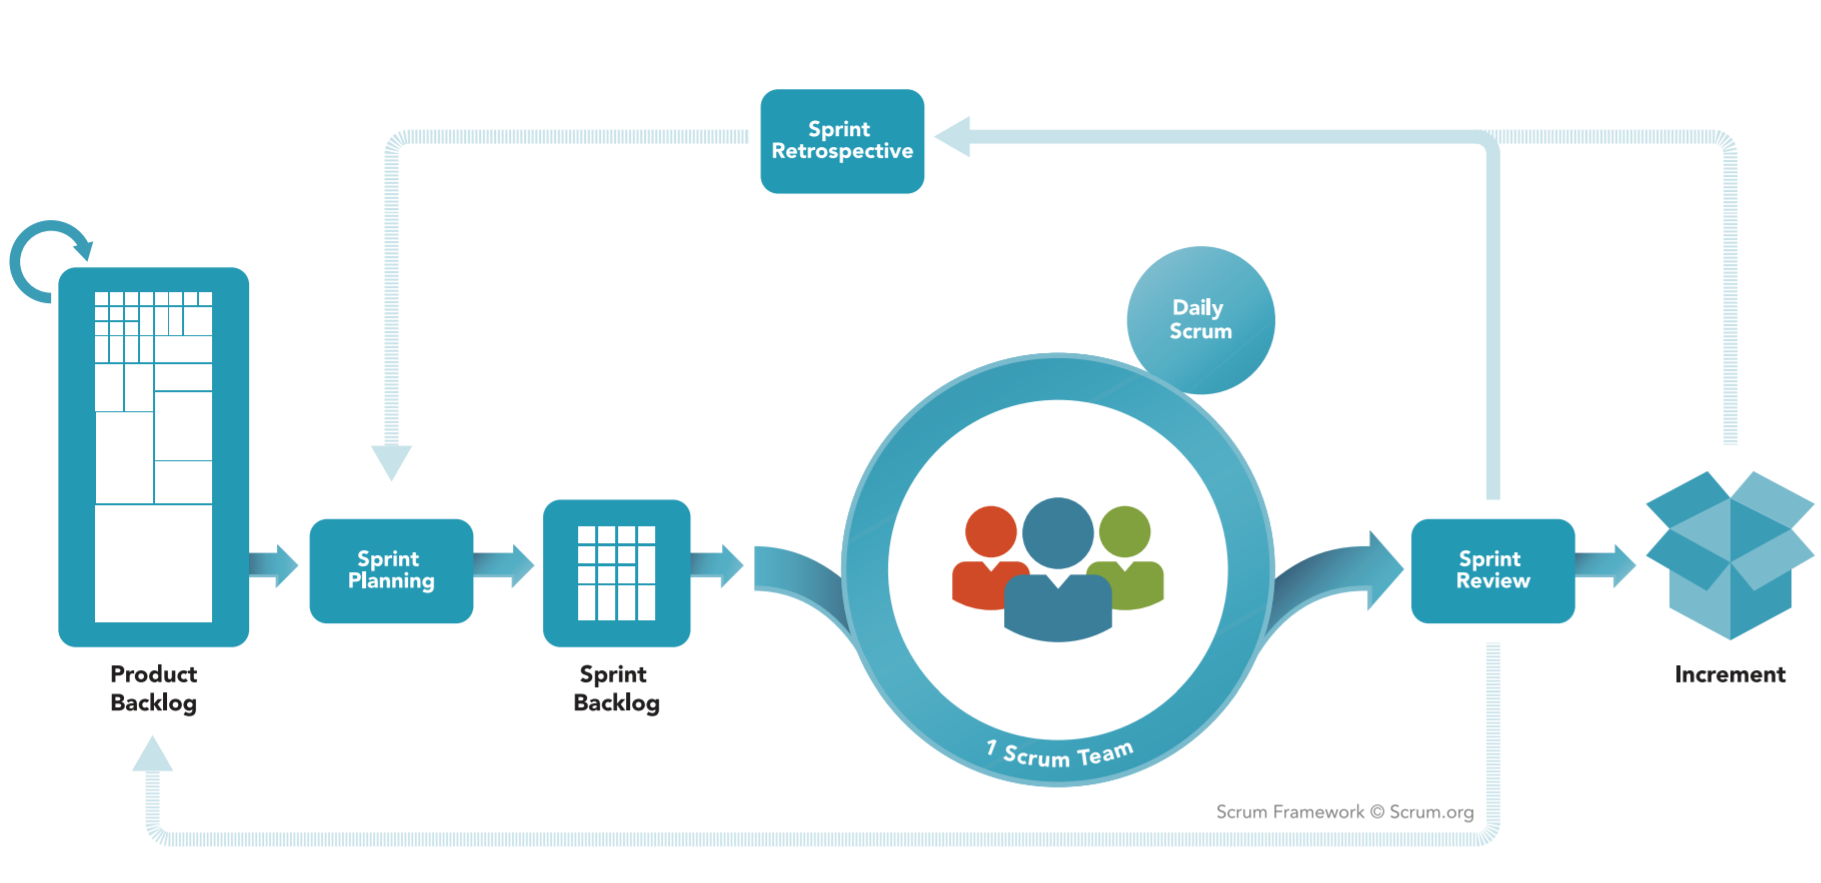
\includegraphics[width=\textwidth] {scrum.jpg}
		\caption{Metodología Scrum }
		\label{fig:scrum}
	\end{figure} 


El proceso comienza con la definición del Product Backlog. De este Product Backlog  se irán obteniendo las historias para los distintos sprints. El proceso general se puede ver en la figura~\ref{fig:scrum}. A continuacion comentaremos sus partes:
\begin{itemize}
\item \textbf{Definición del Product Backlog}. Figura~\ref{fig:product}
Es una lista con las funcionalidad de la aplicación.
Estas funcionalidades que se definen en el Product Owner son las historias del usuario, es decir, es lo que el usuario quiere hacer en la aplicación y por tanto en muchos casos cada historia puede contener varios casos de uso. \\
Está elaborado por el Product Owner y las funcionalidad están ordenadas de mayor a menor importancia para el cliente. La finalidad del Product Owner es plantear lo que hay que hacer.
Con las historias ordenadas se indicarán los Sprints que serán necesarios pudiendo hacer  varias historias en un mismo Sprint pero nunca una historia dividida en dos Sprints. 

 
 \begin{figure}
		\centering
		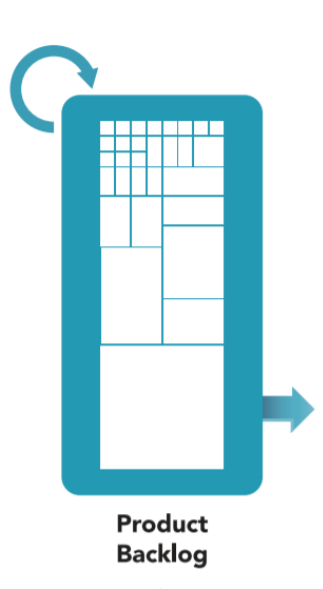
\includegraphics[width=0.2\textwidth] {product.png}
		\caption{Parte metodología Scrum, Product Backlog }\label{fig:product}
	\end{figure} 


\item \textbf{Sprint Planning Meeting}. Figura~\ref{fig:planing}\\
 Esta reunión se hace al comienzo de cada Sprint y se define cómo se va a enfocar el proyecto, se revisan las historias con mayor prioridad y se decide el Sprint backlog.
\begin{figure}[H]
		\centering
		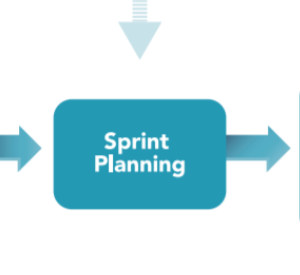
\includegraphics[width=0.3\textwidth] {planing.png}
		\caption{Parte metodología Scrum, Sprint Planning }\label{fig:planing}
	\end{figure} 

\item \textbf{Sprint Backlog}. figura~\ref{fig:sprint}\\
Es el conjunto de historias del Product Backlog que se decidirán hacer en el Sprint, estando ordenadas de mayor a menor prioridad. Una vez completado los miembros del equipo dividirán las historias en tareas más pequeñas y más manejables, si es necesario.

\begin{figure}[H]
		\centering
		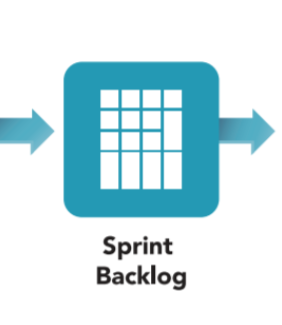
\includegraphics[width=0.3\textwidth] {sprint.png}
		\caption{Parte metodología Scrum, Sprint Backlog }\label{fig:sprint}
	\end{figure} 

 
 
\item \textbf{Daily Scrum o Stand-up Meeting. Figura~\ref{fig:daily}}\\
Es una reunión breve que se realiza cada mañana mientras dura el periodo de Sprint. 
En estas reuniones si algún miembro del equipo encuentra algún problema  se comenta y se trata de buscar la solución. El scrum master es el encargado de lidiar con los inconvenientes encontrados.

\begin{figure}[H]
		\centering
		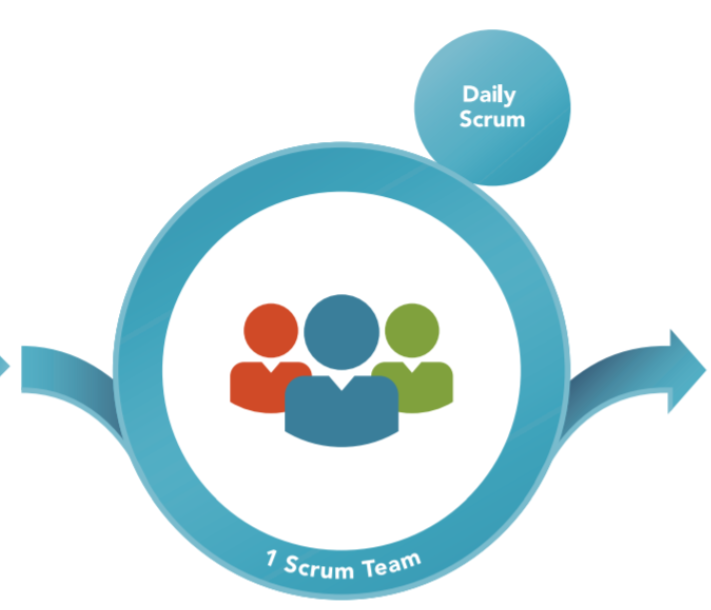
\includegraphics[width=0.3\textwidth] {daily.png}
		\caption{Parte metodología Scrum, Daily Scrum }\label{fig:daily}
	\end{figure} 

\item\textbf{ Sprint Review}\\
Esta sería la primera reunión una vez acabado el Sprint. En ella se deberían plantear las tareas acabadas y se debería ver un avance claro para ser presentado al cliente. Las tareas inacabas las deberían ser devueltas al Product Backlog y si hiciera falta volver a calcular las prioridades.

 \item \textbf{Sprint Retrospective}\\
  El equipo revisa los objetivos cumplidos del Sprint terminado. Se anota lo bueno y lo malo, para no volver a repetir los errores. Esta etapa se centra en el cómo se realiza el proyecto para si hay algún error en el desarrollo poder resolverlo en el siguiente Sprint.
\end{itemize}



\section{Adaptación la metodología a este proyecto }
 Debido a la naturaleza de un Trabajo de fin de grado  debimos realizar una serie de cambios o adaptaciones en ciertos elementos como fueron los siguientes :
\subsection{Participantes}
Los participantes fueron los siguientes:
\begin{itemize}
\item El Product Owner interpretado por los  directores.
\item El cliente tambien fue desempeñado por los directores.
\item El Scrum Master no se usó puesto que se decidió 
 user scrum program.
\item  Y el equipo solo estuvo formado por el alumno.

\end{itemize}

\subsection{Sprints}
Cada sprint siempre tuvo una duración establecida de 4 semanas y 5 horas cada día aunque la carga de trabajo variaba en algún Sprint.


\subsection{Reuniones}

En el apartado de las reuniones siempre se establecían las tareas a realizar en cada jornada de trabajo. Al finalizar cada Sprint se realizaban reuniones con los directores y se aprovechaba para la planificación de la siguiente.\\

Una vez adaptada la metodología a este proyecto encontramos las siguientes ventajas a su uso:

\begin{itemize}
\item Ayuda a estar más centrado en el producto durante el desarrollo del proyecto ya que no existe la preocupación por establecer las siguientes tareas.  Estas ya quedaron indicadas en el sprint. 



\item En ocasiones al ir avanzando en el desarrollo aparecen nuevas funcionalidades que se pueden ir añadiendo al Product Backlog. Esto lo podemos hacer siempre y cuando nos ciñamos al Sprint Backlog
 para saber la tarea que realizar en ese momento.


\item  Las historias de usuario se irán dividiendo en tareas que se puedan realizar durante el sprint. De este modo una vez acabado el sprint tengamos un producto potencialmente entregable.\\

Dado el poco conocimiento de la metodología Scrum antes de la realización del proyecto, el ir avanzando en el proceso ayuda a adquirir conocimientos. Los cuales ayudarán a estimar mejor la duración e importancia de los elementos que se añaden al Sprint Backlog.


\item
Durante el desarrollo del proyecto hay ciertas funcionalidades que pueden cambiar. Empleando los principios de las metodologías ágiles en cada iteración haremos que el proyecto sea mas adaptable antes nuevos requisitos y cambios.

\end{itemize}

		\cleardoublepage

\chapter{Analisis}
		\label{dev}
		\input{subfiles/análisis}
		\cleardoublepage

\chapter{Diseño}
		\label{dis}
		\input{subfiles/diseño}
 		\cleardoublepage



\chapter{Conclusiones y trabajo futuro}
        \label{conc}
        

\section{Trabajo realizado}
Una vez finalizado este Proyecto de Fin de Grado tenemos una aplicación móvil en Android que cumple todos los objetivos marcados al inicio del proyecto y en especial de esta memoria. La aplicación permitirá al usuario gestionar sus grupos, gestionar sus puntos de interés y guardar sus rutas tantos las que hace de manera individual como las que hace de manera conjunta. Esto último lo hace gracias al sistema de localización del GPS.\\


A continuación se muestran las principales características del producto construido: 

\begin{itemize}
\item Registrarse para poder disfrutar de las funcionalidades que ofrecemos y llevar un seguimiento de sus actuaciones en el campo.
\item Guardar puntos estratégicos en el mapa acompañados de un nombre clave y una breve descripción. Esto nos ayudará a recordar puntos para futuras aventuras. 
\item Crear grupos de compañeros y poder añadirlos para compartir rutas.
\item Guardar las rutas seguidas en nuestras aventuras de pesca y de caza, como también la posibilidad de rememorar esas rutas al poder revisarlas gracias a nuestras lista con las rutas seguidas.
\item Y por último la posibilidad de realizar rutas conjuntas con un grupo de amigos que nosotros queramos y así compartir nuestra ubicación en todo momento. Esto nos ayudará en la pesca ya que al conocer la ubicación del resto de integrantes del grupo podríamos socorrerlo si algo le pasa en un sitio de difícil acceso. Como también por tema de seguridad en una jornada de caza ya que si estamos cerca de otro usuario lo veríamos.
\end{itemize}  

\section{Trabajo futuro}
 La aplicación cumple con los objetivos marcados pero como todo proyecto software puede ser ampliado y mejorado. Una vez finalizado este proyecto, se podrían añadir nuevas funcionalidades:



\begin{itemize}
\item Añadir nuevos tipos de PDIs como es el caso de fotografía. Ya que tiene varias semejanzas con la caza y la pesca por los lugares donde se realiza sería una funcionalidad interesante.
\item Como toda actividad que se realiza al aire libre esta condicionada para bien o para mal por condiciones meteorologías, se podrían usar los servicios de OpenWeatherMap. Esto nos ayudaría a planear mejor nuestras jornadas de pesca, caza o fotografía.


\item Otro punto interesante también sería poder añadir a cada PDI una foto asociada a él, lo que ayudaría a acordarse mejor del lugar y ubicarse con precisión.
\end{itemize}

        \cleardoublepage

\listoftables
\cleardoublepage

\listoffigures
\cleardoublepage

%%%%%%%%%%%%%%%%%%%%%%%%%%%%%%%%%%%%%%%%
% Apéndices
%%%%%%%%%%%%%%%%%%%%%%%%%%%%%%%%%%%%%%%%
\appendix
\addcontentsline{toc}{chapter}{Apéndices}

\chapter{Glosario}
		\label{glosario}
		
\renewcommand*{\arraystretch}{1.5}
\begin{description}
\item{





\end{description}
		\cleardoublepage

\cleardoublepage


%%%%%%%%%%%%%%%%%%%%%%%%%%%%%%%%%%%%%%%%
% Bibliografía
%%%%%%%%%%%%%%%%%%%%%%%%%%%%%%%%%%%%%%%%
\bibliographystyle{alpha}
\bibliography{references}
\end{document}


